\documentclass[../main.tex]{subfiles}
\begin{document}

\section{Introduction}
\epigraph{The problem of learning is arguably at the very core of the problem of intelligence, both biological and artificial}{\textit{Poggio, Shelton, AI Magazine 1999}}
\subsection{What is ML}
 The field of \textbf{machine learning} is concerned with the question of how to construct computer programs that automatically improve with experience. \\
In recent years many successful machine learning applications have been developed, ranging from data-mining programs that learn to detect fraudulent credit card transactions, to information-filtering systems that learn users' reading preferences, to autonomous vehicles that learn to drive on public highways. \\
At the same time, there have been important advances in the theory and algorithms that form the foundations of this field. Machine learning draws on concepts and results from many fields, including statistics, artificial intelligence, philosophy, information theory, biology, cognitive science, computational complexity, and control theory.

 \textbf{Machine Learning} has emerged as an area of research combining the aims of \textit{creating computers that could learn} (AI - Build adaptive/personalized intelligent systems) and new powerful \textit{adaptive/statistical tools} with rigorous foundation in computational science for data analysis.\\
\textbf{Learning} is the major challenge and a strategic way to provide intelligence into the systems.

\theoremstyle{definition}
\begin{definition}[Learning Computer]
A computer program is said to \textbf{learn} from experience \textit{E} with respect to some class of tasks \textit{T} and performance measure \textit{P}, if its performance at tasks in \textit{T}, as measured by \textit{P}, improves with experience \textit{E}.
\end{definition}

The ML studies and proposes methods to build (infer) a model (dependencies / functions / hypotheses) from examples of observed data
\begin{itemize}
    \item That fits the known examples.
    \item Able to generalize with reasonable accuracy for new data (according to verifiable results, under statistical and computational conditions and criteria).
    \item Considering the expressiveness and algorithmic complexity of the models and learning algorithms.
\end{itemize}
\begin{example}[Inferring general functions from know data]
Two famous examples of ML tasks:
\begin{itemize}
    \item Handwriting Recognition: $x$ (Data from pen motion) and $f(x)$ (Letter of the alphabet)
    \item Face recognition: $x$ (Bitmap picture of person's face) $f(x)$ (Name of the person)
\end{itemize}   
\end{example}

So we have some opportunity (if useful) and awareness (needs and limits):

\textbf{Utility of predictive models: (in the following cases)}:
\begin{itemize}
    \item no (or poor) theory (or knowledge to explain the phenomenon)
    \item uncertain, noisy or incomplete data (which hinder formalization of solutions)
\end{itemize}

\textbf{Requests}:
\begin{itemize}
    \item source of training experience (representative data)
    \item tolerance on the precision of results
\end{itemize}

\subsection{Overview: Components of a ML System}
Main components of a ML system, Framework as a guide to the key design choices:
 
\begin{figure}[ht!]
\centering
\includegraphics[scale=0.3]{lectures/1_Introduction/comp.png}
\caption{Components of a ML system}
\label{fig:MLComponents}
\end{figure}

\subsection{Data}
The data represent the available facts (experience). Representation problem: to capture the structure of the analyzed objects. \textbf{Type}: Flat, Structured, ...

\noindent We will generally use flat data:\\
 E.g. \textbf{Flat DATA} (attribute-value language): fixed-size vectors of properties (features), single table of tuple (measurements of the objects), Attributes can be discrete or continuous

\begin{figure}[H]
\centering
\includegraphics[scale=0.4]{lectures/1_Introduction/flat_data.png}
\end{figure}
Of course Data type can be different, usually there is a Data Preprocessing step, e.g. Variable scaling, encoding, selection...
For this step, see in Data Mining: \textit{Data Understanding} and \textit{Data Preparation}.

\noindent\textbf{Example and terminologies}\\
Let's see a example with some Medical records in the flat case: 

\begin{figure}[H]
\centering
\includegraphics[scale=0.4]{lectures/1_Introduction/flat_data_medical.png}
\end{figure}

\begin{itemize}
    \item Each row ($\mathbf{x}$, vector): example, pattern, instance, sample,...
    \item Dimension of data set: number of examples $l$
    \item Dimension (of $\mathbf{x}$): number of features $n$
    \item If we will index the features/inputs/variables by $j$ : 
	variable $x_j$ is (typically) the j-th \\ feature/property/attribute/element of $\mathbf{x}$.
\end{itemize}
but may be to simplify we need to use subscript index for other meanings
\begin{itemize}
    \item $\textbf{x}_p$ is (typically) the p-th pattern/example/raw ($\textbf{x}$ bold is a vector)
    \item $x_{pj}$ for example can be the attribute j of the pattern p
\end{itemize}

\noindent\textbf{DATA Encoding}\\
For the \textbf{Flat case} we can have \textbf{Numerical encoding for categories} e.g.:
\begin{itemize}
    \item 0/1 (or –1/+1) for 2 classes
    \item 1,2,3... Warning: grade of similarity (1 vs 2 or 3): useful for “order
categorical” variables (e.g small, medium, large)
    \item 1-of-k (or 1-hot) encoding: useful for symbols

    \begin{figure}[H]
    \centering
    \includegraphics[scale=0.45]{lectures/1_Introduction/data_encoding.png}
    \end{figure}
    This is useful because the scalar product between two vectors representing two coded symbols is zero. The vectors are orthogonal, this implies that there is no relation between the category symbols.
\end{itemize}

\noindent Another types of Data:\\
\noindent E.g. \textbf{Structures DATA}: Sequences (lists), trees, graphs, Multi-relational data (table) (in DB)\\
Examples: images, microarray, temporal data, strings of a language, DNA e proteins, hierarchical relationships, molecules, hyperlink connectivity in web pages, ...

\noindent\textbf{Further terminologies}
\begin{itemize}
    \item \textbf{Noise}: addition of external factors to the stream of target information (signal); due to randomness in the measurements, not due to the underlying law: e.g. Gaussian noise
    
    \begin{figure}[H]
    \centering
    \includegraphics[scale=0.2]{lectures/1_Introduction/sig_noise.jpg}
    \end{figure}

    \item \textbf{Outliers}: are unusual data values that are not consistent with most observations (e.g. due to abnormal measurements errors). Some operation can be perform: outlier detection and preprocessing (removal) or we have to use some Robust Modeling Methods.
    \item \textbf{Feature selection}: selection of a small number of informative features: it can provide an optimal representation for a learning problem
\end{itemize}

\subsection{Task}
The task defines the purpose of the application: Knowledge that we want to achieve? Which is the helpful nature of the result? What information are available?\\
There are two main categories of tasks:
\begin{itemize}
    \item \textbf{Predictive} (Classification, Regression): function approximation (build a function from examples)
	\begin{figure}[H]
	    \centering
	    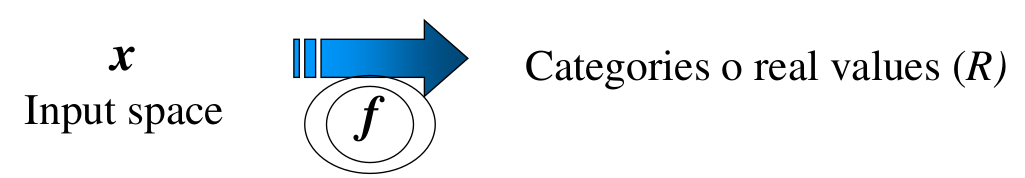
\includegraphics[width=0.8\textwidth]{lectures/1_Introduction/task_pred.png}
	    \label{fig:task-scheme}
	\end{figure}
    \item \textbf{Descriptive} (Cluster Analysis, Association Rule): find subsets or groups of unclassified data
\end{itemize}
We can usually divide tasks in \textit{Supervised Learning} and \textit{Unsupervised Learning}:

\subsubsection*{Supervised Learning}%
Given a training example as $<input,output>=<\textbf{x},d>$ (\textbf{labeled example}) for an unknown function $f$, the aim is to find a \emph{good} approximation to $f$ (an \textbf{hypothesis} $h$ that can used for prediction on unseen data \textbf{x'}).\\
Target $d$ (or $t$ or $y$) is given by the teacher according to a $f(\mathbf{x})$ (unknown function), $d$ is usually a numerical/categorical label:
\begin{itemize}
    \item \textit{Classification}: discrete value outputs: 
	\[
    	f(\mathbf{x}) \in \{1, 2, \dots, K\} \; \; \text{classes (discrete-valued function)}
	.\] 
    \item \textit{Regression}: real continuous output values (approximate a real-valued
target function)
\end{itemize}
Note: we can use the same model, we only have to change the domain of the output (Unified vision thanks to the formalism of func. approximation).

\subsubsection*{Unsupervised Learning}%
Given a training set of \textbf{unlabeled data} $<\textbf{x}>$, the aim is to find a \emph{natural groupings} in the set.
Some taks are:
\begin{itemize}
    \item Clustering, see figure \ref{fig:intro_clusterinng_exp}
    \item Dimensionality reduction/ Visualization/Preprocessing
    \item Modeling the data density
\end{itemize}
\begin{figure}
    \centering
    \includegraphics[scale=0.5]{lectures/1_Introduction/clustering.png}
    \caption{An Example of Clustering, Partition of data into clusters (subsets of “similar” data)}
    \label{fig:intro_clusterinng_exp}
\end{figure}
\subsubsection{Classification}
(Supervised) Classification: Patterns (features vectors) are seen as members of a class and the goal is to assign the patterns observed classes (label). \\
So, the aim is to find a \emph{good} approximation to $f(\textbf{x})$ (an \textbf{hypothesis} $h$) that can be used to return a prediction on unseen data \textbf{x'} and tell what class \textbf{x'} belongs to, see figure \ref{fig:intro_classification_exp1}.

If the number of classes is 2, the approximation of $f(\textbf{x})$ is a boolean function (binary classification, \textbf{concept learning}), instead if the number of classes is greater than 2, we talk about \emph{multi-class problem} $(C_1, C_2, \dots, C_k)$.

\begin{figure}
    \centering
    \includegraphics[scale = 0.5]{lectures/1_Introduction/intro_classification_1.png}
    \caption{A classification task: we want to get an approximation to $f(\mathbf{x})$, we want to understand if future patients are positive or negative to a certain diagnosis}
    \label{fig:intro_classification_exp1}
\end{figure}

The classification may be viewed as the allocation of the input space in decision regions (e.g. 0/1) and we want to find a linear separator on an instance space $\mathbf{x} = (x_1, x_2) \text{in } \mathbb{R}^2$ where $f(x)= 0/1 (\text{or } -1/+1 )$. 

\begin{figure}[ht]
  \centering
  \subfloat[Separating (hyper)plane : $x$.]{\includegraphics[width=0.5\textwidth]{lectures/1_Introduction/classification.png}\label{fig:f1}}
  \hfill
  \subfloat[Geometrical 3D view: classifier]{\includegraphics[width=0.5\textwidth]{lectures/1_Introduction/intro_classification_2.png}\label{fig:f2}}
  \caption{An example of classification, that use a linear separator on the instance space.}
\end{figure}
In figure \ref{fig:f1} we can see an hyperplane which separates the points and this is a hypothesis $h(x)$ (an approximation to $f(\mathbf{x})$) found in the space of hypotheses $H$ (set of dichotomies induced by hyperplanes), see figure \ref{fig:intro_classification_exp2}.
\begin{figure}[H]
    \centering
    \includegraphics[scale = 0.4]{lectures/1_Introduction/intro_classification_3.png}
    \caption{Hyperplanes classifier}
    \label{fig:intro_classification_exp2}
\end{figure}


\newpage
\subsubsection{Regression}
    Process of estimating of a real-value function on the basis of finite set of noisy samples (supervised task), we have known pairs $(x, f(x)+\text{random noise})$.\\
    \textbf{Goal Task}: find a function that approximate the data in figure \ref{fig:intro_regression_exp1}:
    \begin{figure}[H]
        \centering
        \includegraphics[scale = 0.3]{lectures/1_Introduction/intro_regression_exp1.png}
        \caption{A example of regression }
        \label{fig:intro_regression_exp1}
    \end{figure}
    Regression: $x =$ variables (e.g real values), ($f(x)+\text{random noise}$) real values that we know, so we want to find a curve that best fit the data: \textit{curve fitting}.
    \begin{figure}[ht]
        \centering
        \includegraphics[scale = 0.4]{lectures/1_Introduction/regression.png}
    \end{figure}
    An example of curve fitting is a \textbf{linear hypothesis}: $h_w(x) = w_1x + w_0 = 0.2x-0.4$ but we have to choose the best one with some criteria.

\subsubsection{Other Tasks}
There are other types that we will not discuss, like:
\begin{itemize}
    \item \textbf{Dimensionality reduction} (in unsupervised Learning)
    $$ <x_1, x_2, \; \dots, x_n> \; \rightarrow \; <x_1, x_2, \; \dots, x_m> \; \text{with } m < n  $$
    
    \item \textbf{Reinforcement Learning}(learning with right/wrong critic):
    This is usually a supervised learning task with some police!
    \begin{figure}[H]
        \centering
        \includegraphics[scale = 0.6]{lectures/1_Introduction/Reinforcement_Learning.png}
    \end{figure}

    \item \textbf{Semi-supervised learning}: combines both labeled and unlabeled examples to generate an appropriate function or classifier.
\end{itemize}

\subsection{Models}
The aim is to capture/describes the relationships among the data (on the basis of the task) by a “language”. The “language” is related to the representation used to get knowledge. It defines the class of functions that the learning machine can implement (\emph{hypothesis space}). \\
E.g. set of functions $h(x,w)$, where $w$ is the (abstract) parameter.

\begin{definition}[Model main terms]
The terminologies associated to the model is:
\begin{itemize}
    \item \textbf{Training examples} (supervised learning):\\
    An example of the form $(x, f(x))$. $x$ is usually a vector of features, $t=f(x)$ is called the target value.
    \item \textbf{Target function}: The true function $f$ (that we don't have! we want to approximate it!)
    \item \textbf{Hypothesis}: A proposed function $h$ believed to be similar to $f$. An expression in a given \emph{language} that describes the relationships among data.
    \item \textbf{Hypotheses space (H)}: The space of all hypotheses that can, in principle be output by the learning algorithm (set of functions $h(x,w)$, where $w$ is the parameter), this is a Hilbert Space.
\end{itemize}   
\end{definition}


Some models are shown here:
\begin{figure}[H]
    \centering
    \includegraphics[scale = 0.4]{lectures/1_Introduction/intro_trivial_model_eg.png}
\end{figure}

Another example: we will see a \textbf{neural networks}, beyond the neurobiological inspiration, as a computational model for the treatment of data, capable of approximating complex (non-linear) relationships between inputs and outputs.
\begin{figure}[H]
    \centering
    \includegraphics[scale = 0.35]{lectures/1_Introduction/intro_nn.png}
\end{figure}
\subsubsection{Pardigms and methods (Languages for H)}
\begin{itemize}
    \item Symbolics and Rule-based (or discrete H)
    \begin{itemize}
        \item Conjuction of literals, Decision trees (propositional rules)
        \item Inductive grammars, Evolutionary algorithms, …
        \item Inductive Logic Programming (first order logic rules)
    \end{itemize}
    \item Sub-symbolic (or continuous H)
    \begin{itemize}
        \item Linear discriminant analysis, Multiple Linear Regression, LTU
        \item Neural networks
        \item Kernel methods (SVMs, gaussian kernels, spectral kernels, etc)
    \end{itemize}
    \item Probabilistic/Generative
    \begin{itemize}
        \item Traditional parametric models (density estimation,discriminant analysis,polynomial regression,...)
        \item Graphical models: Bayesian networks,naive Bayes, PLSA, Markov models, Hidden Markov models, ...
    \end{itemize}
    \item Instance-based
    \begin{itemize}
        \item Nearest neighbor
    \end{itemize}
\end{itemize}

\subsubsection{How many models?}
\begin{theorem}[No Free Lunch Theorem]
There is no universal “best” learning method (without any knowledge, for any problems,...): if an algorithm achieves superior results on some problems, it must pay with inferiority on other problems. In this sense there is no free lunch.
\end{theorem}
\textbf{NOTE}: However, not all the models are equivalent: (instead of assuming a specific form for the target function (parametric models in classical Statistics)).\\
The course provide: 
\begin{itemize}
    \item A set of models.
    \item The critical instrument to compare them.
\end{itemize}
 

The core of ML is on flexible approaches that can in principle approximate arbitrary functions (universal approximation property).

\textbf{NOTE}: Typical powerful models of ML are Neural Networks, always remeber that “power is nothing without control”: we need of inductive principia for the control of the complexity.

\subsection{Learning Algorithms}
A Learning Algorithms is basing on data, task and model!\\
(Heuristic) search through the hypothesis space \emph{H} ($h \in \emph{H}$) of the \textbf{best hypothesis} (Typically searching for the h with the minimum “error”, the best approximation to the unknown target function). Practically we want to find parameters $w$ that give the best $h$.

\begin{example}
    Learning could mean to search the best $\boldsymbol{w}$  for the linear models or best rules for symbolic model.
\end{example}

\emph{H} may not coincide with the set of all possible functions and the search can not "be exhaustive": it needs to make assumptions (we will see the role of \emph{Inductive bias}), see figure \ref{fig:lern_search}.

\begin{figure}[ht]
    \centering
    \includegraphics[scale = 0.35]{lectures/1_Introduction/intro_search.png}
    \caption{(Local) search on the hypothesis space: each point is a function, we set an initial condition and we move to a set of optimal solution (red).}
    \label{fig:lern_search}
\end{figure}

\noindent \textbf{Learning (terminologies)}:
According to the different paradigms/contexts “learning” can be differently termed or have different acceptations:
\begin{itemize}
    \item Inference (statistics)
    \item Inference: Abduction/Induction (logic)
    \item Adapting (biology, systems)
    \item Optimizing (mathematics)
    \item Training (e.g. Neural Networks)
    \item Function approximations (mathematics)
\end{itemize}

\noindent Can be more specifically found in other sub-fields:
\begin{itemize}
    \item Regression analysis (statistics), curve fitting (math, CS), ...
    \item Or using other terminologies e.g. “Fitting a multivariate function”
\end{itemize}

\subsection{Role of inductive bias}%
In order to set up a model and a learning algorithm we can make
assumptions (about the nature of the target function) concerning either
\begin{description}
    \item[Language bias] Constraints in the model (in the hypothesis space H, due to the set of
	hypotheses that we can express or consider). For example we can search only on linear function.
    \item[Search bias] Constraints or preferences in learning algorithm/search strategy. For example we could choose to search only some $\boldsymbol{w}$ for the linear search.
    \item[Both] Search bias and inductive bias together.
\end{description}
Such assumptions are strictly need to obtain an useful model for the ML aims ( a model with generalization capabilities ).\\
We start to discuss it within examples in discrete hypotheses spaces (rules) , learning a concept (a Boolean function) [Mitchell chapt. 2]
\begin{example}[A simple rule]
    $x$ is a “cat” if $h_{cat}( x ) =1$, otherwise is $0$ for $x$ in “animals”
\end{example}

\paragraph{Learning a Boolean function}%
Given a space of boolean variable $x_i$ we can create a number of boolean function equal to $2^{2^n}$. 
\begin{example}
  Given 4 boolean variable $x_i$, $i = 1,\ldots, 4$ we search in the space of the combination of all possible output.
  \begin{figure}[H]
      \centering
      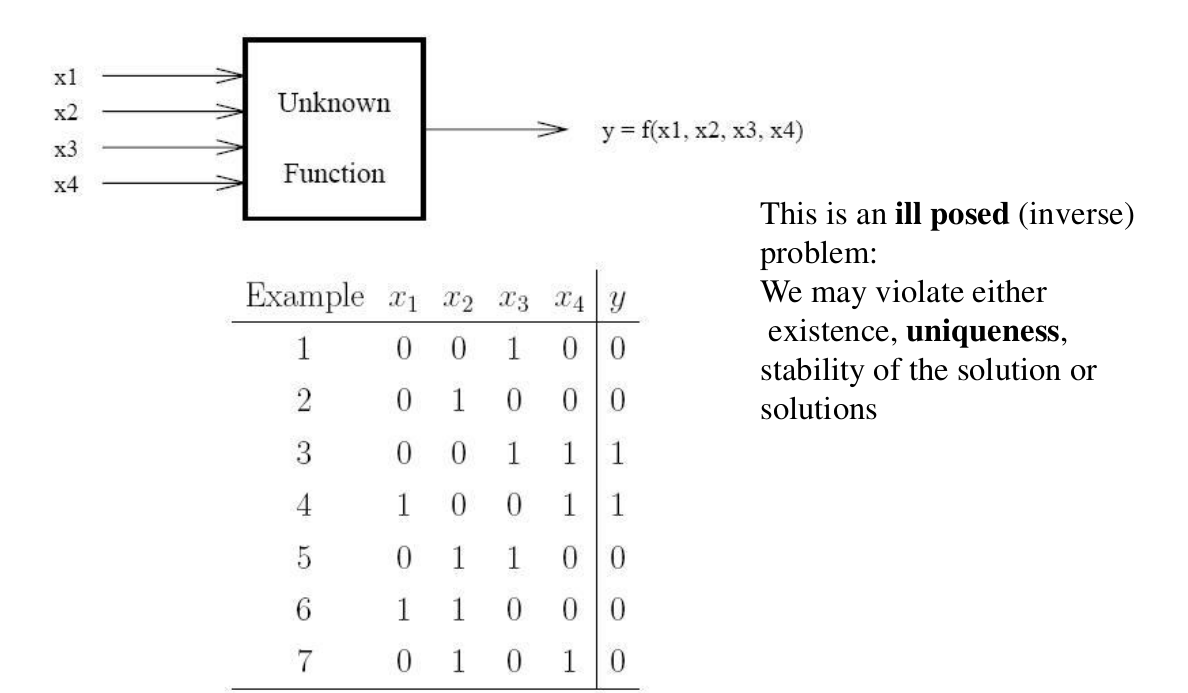
\includegraphics[width=0.8\textwidth]{lectures/1_Introduction/learn_bool_func.png}
  \end{figure}
  In the table there aren't all the possible combinations of the $x_i$, only 7 examples are given. The task is to infer the output for the other 9 combination but\ldots There are still $2^9$ combination of function that agree with the provided examples! ($2^9 = 2^{16 - 7})$.
\end{example}
This kind of problem is ill posed so the uniqueness of solution is not guaranteed. A learner of this type is called Rote Learner.
\begin{definition}[Rote Learner]
    A rote learner is a learning algorithm that stores examples and classify new instances only if they match with a previous observed example.
    If a new instance doesn't match with any of the preceding instance the rote learning just classify as "I don't know".
\end{definition}

\paragraph{Cunjuctive Rules}%
As second example of discrete \textit{Hypotesys Space H} we could imagine to learn a discrete function with discrete inputs assuming cunjunctive rules.
\begin{example}
Take this 3 proposition: $l_1 = $"the animal is furry", $l_2 = $"the animal purrs", $l_3=$"the animal is a cat". \\
The conjunctive rule could be: if ($l_1$ and $l_2$)=True than $l_3=$True, else $l_3=$False. \\
So the function $h$ is:
\[
    h(l_1, l_2, l_3) = 
    \begin{cases}
	l_3 & \text{if } l_1 \text{ and } l_2\\
	\text{not }l_3 & \text{otherwise}
    \end{cases}
\] 
\end{example}
In this space, given $n$ proposition we can have $3^n + 1$ semantically distinct \textit{Hypoteses} (conjunctions): 
\begin{itemize}
    \item $l_i$.
    \item not $l_i$.
    \item Don't care.
\end{itemize}
We add the +1 because all the $h$ like $(l_i$ and not $l_i$) are equivalent to false.

\subsubsection{Unbiased Learner}%
\begin{definition}[Consistent Hypotesis]
    An hypotesis is consistent with the training set TR if $h(\boldsymbol{x}) = d(\boldsymbol{x})$ for each training sample $\left<\boldsymbol{x}, d(\boldsymbol{x}) \right>$.
\end{definition}
\begin{definition}[Version Space]
    The version space VS$_{H, TR}$ is the subset of Hypoteses (respect to the Hypotesis space $H$) consistent with all the training sample of the training set TR.
\end{definition}
The version space can be found by clever algorithm described in the book (Mitchell chap. 2).\\
Using only the conjunctive assumption, like in the previous example, may be too restrictive: if the target concept (or function) is not in $H$ it cannot be represented in $H$.
\begin{example}[outside target]
    If ($x_1 = 1$ or $x_2 = 1$) then $h(\boldsymbol{x})=1$ else $h(\boldsymbol{x})= 0$.\\
    With this Hypotesis space we cannot represent $x_i = 0$.
\end{example}
In order to handle this problem we can choose $H$ that express every teachable concept (among proposition). In the conjunctive rules we could choose:
\[
    H = \text{disjunctions}, \text{ conjunctions}, \text{ Negations}.
\] 
In this way $H$ will surely contains the target concept: in this case $H$ will be an \textbf{Unbiased Learner}. 

\subsubsection{Is an unbiased learner good for Generalization?}%
The only example that are unanbigously classified by an unbias learner (represented with the VS) is are the training examples themselves.

\begin{theorem}[About unbiased learner]
    An unbiased learner is unable to Generalize (on new instances).
\end{theorem}
\begin{proof}
    Each unobserved instance will be classified positive by precisely half the hypothesis in VS and negative by the other half ( rejection: no answer is made by the VS for new input instances).\\
    Indeed, given $x_i$ in the test set:\\
    $\forall h$ consistent with $x_i$ $\exists h'$ identical to $h$ except $h'(x_i) \neq h(x_i)$, $h' \in $ VS and $h \in $ VS.
\end{proof}
So a learner that makes no prior assumptions regarding the identity of the target function/concept has no rational basis for classifying any unseen instances.

\textbf{Important}: bias is not only assumed for efficency but it is \textbf{needed} for the generalization capability.

\subsubsection{Inductive or Deductive System}%
Inductive systems are equivalent to deductive systems if we insert in our hypotesis the inductive bias. In this way the problem about the classification of new instance makes sense: doing ML we are not inveting crazy useless functions.
\begin{figure}[H]
    \centering
    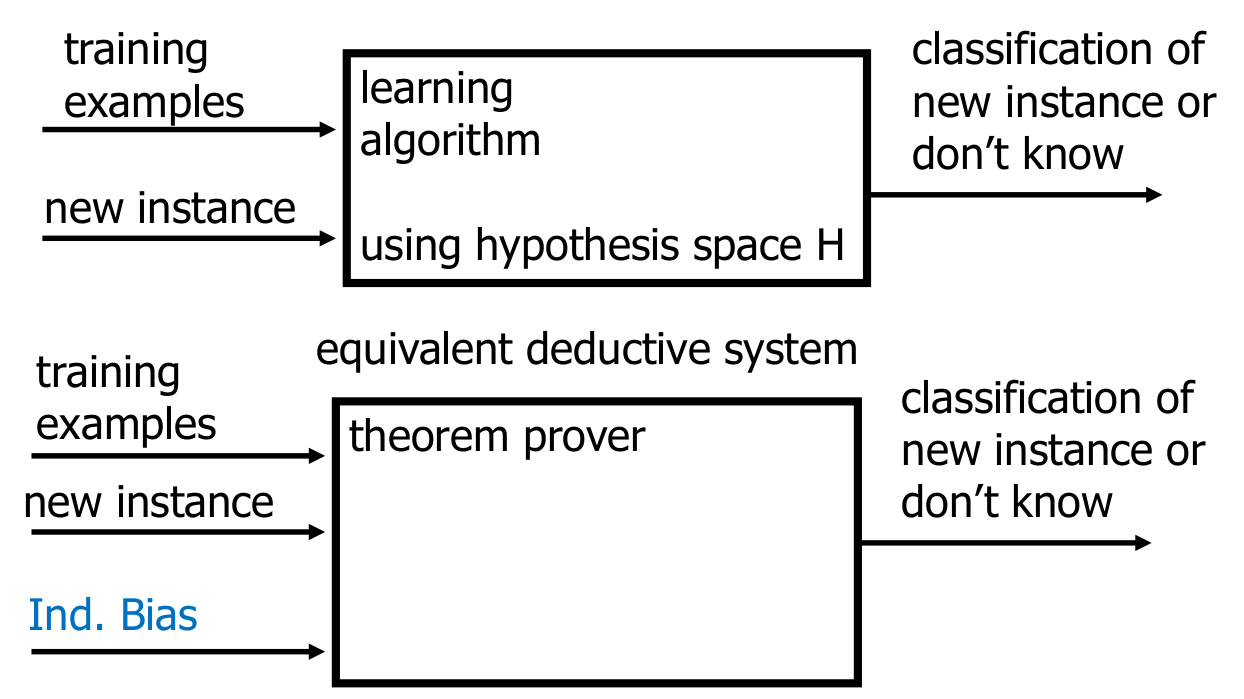
\includegraphics[width=0.5\textwidth]{lectures/1_Introduction/dedu_indu_sys.png}
\end{figure}

\subsubsection{Language or Search bias?}%
In ML is typically used a flexible approaches (expressive hypothesis spaces, universal capability of the models, e.g. Neural Networks, DT).\\
Usually we avoid the language bias, hence without excluding a priori the unknown target function. We retain an inductive bias but focusing on the search bias (which is ruled by the learning algorithm).\\
In practice we will use an incomplete search strategy.

\textbf{Conclusions}:
\begin{itemize}
    \item Learning without bias cannot extract any regularities from data (lookup-table: no generalization capabilities).
    \item Every state-of-the-art ML approach shows an inductive bias.
    \item Issue: characterize the bias for different models/learning approaches\ldots Is an Inductive Bias better than another?
\end{itemize}

\subsection{Task + Model = Loss}
We have to find a  “\textbf{good}” approximation to f from examples. How to measure the quality of the approximation?

\noindent We want to measure the “distance” between $h(x)$ (output of the model for input $\mathbf{x}$) and $d$.
\begin{center}
\textit{Minimization of errors in training, check of errors in test}\\
\end{center}
\noindent We will use:
\begin{itemize}
    \item \emph{Loss function}: $L(h(\textbf{x}),d)$ (high value means poor approximation)
    \item The Error (or Risk) is an expected value of the loss:
	\[
	    \text{\emph{Empirical Risk}}: R_{emp}= \frac{1}{l} \sum_{i=1}^{l} L(h(\textbf{x}_i),d_i)
	.\] 
    e.g. a “sum” or mean of the loss over the set of samples.
\end{itemize}
We will change the loss function $L$ for different tasks.

\subsubsection*{Common Tasks review}%
A possible classifications of common learning tasks specifying the (changing of the) nature of the loss function, output and hypothesis space.
\begin{itemize}
    \item Survey of common learning tasks
    \item Nature of models (hypothesis spaces) for different class of tasks.
\end{itemize}

\subsubsection{Loss Function example: Regression}
In a regression task we want to predict a numerical value. We have an \textbf{Hypothesis Space} $H$ that is a set of real-valued functions and the \textbf{Loss function} will measures the approximation accuracy/error between $h(x_i)$ and $d_i = f(x_i) + e$ (real value function + random error).

A common loss function for Regression (predicting a numerical value) is the \emph{squared error}: 
\[
 L(h(\textbf{x}_{i}),d_{i}) = (d_{i} - h(\textbf{x}_{i}))^{2}   
.\] 
We use that error because we want the distance and a negative or positive value makes no different).
\begin{center}
    $R_{emp}$: the mean over the data set provide the \emph{Mean Square Error} (MSE)
\end{center}
\begin{figure}[ht]
    \centering
    \includegraphics[scale=0.4]{lectures/1_Introduction/mse.png}
\end{figure}

\subsubsection{Loss Function example: Classification}
Classification of data into discrete classes, $d_i$ can be e.g. $0/1$ and $h(x_i)$ will predict $0/1$. So our \textbf{Loss Function} will measures the classification error:

\[
    L(h(\textbf{x}_{i}),d_{i}) = \left\{
                \begin{array}{ll}
                  0 \quad if \;\;h(\textbf{x}_{i}) = d_i\\
                  1 \quad otherwise
                \end{array}
              \right.
\]
 
\begin{center}
    $R_{emp}$: The mean over the data set provide the number/percentage of misclassified patterns
\end{center}
\begin{example}
    20 out of 100 are misclassified $\rightarrow$ 20\% errors, i.e. 80\% of accuracy
\end{example}

\subsubsection{Loss Function example: Clustering and Vector Quantization}
\textbf{Goal}: optimal partitioning of unknown distribution in x-space into regions (clusters) approximated by a cluster center or prototype. e.g see figure \ref{fig:intro_clusterinng_exp}

\noindent \textbf{H}: a set of vector quantizers $ x \rightarrow c(x) \;\;( \text{continuosspace} \rightarrow \text{discrete space})$

\noindent \textbf{Loss Function}: would be the squared error distortion:
$$L(h(\textbf{x}_{i})) = \langle\,(\mathbf{x}_i - h(\mathbf{x}_i))\,, (\mathbf{x}_i - h(\mathbf{x}_i))\rangle \quad \text{( inner product )}$$

Proximity of the pattern to the centroid of its cluster

\subsubsection{Loss Function example: Density estimation}
Density estimation (generative, “parametric methods”) from an assumed class of density
\begin{figure}[H]
    \centering
    \includegraphics[scale = 0.4]{lectures/1_Introduction/intro_density_estimation.png}
\end{figure}



\subsection{GENERALIZATION}
Learning: search for a good function in a function space from known data (typically minimizing an Error/Loss), but how we can say that this model is good for our task after the learning step?

\textbf{Note}: This is the answer for the question: "What's the meaninng of Machine Learning?"
\begin{center}
    A model is Good with respect to the \textbf{generalization error}: how accurately the model predicts over novel samples of data (Error/Loss measured over new data) 
\end{center}

So \textit{Generalization} is a crucial point of ML. We will see the difference between "Easy to use ML tools" and the "correct/good use of ML".

So we have two main phases:
\begin{itemize}
    \item \textbf{Learning} phase \textbf{(training, fitting)}: build the model from know data – \emph{training data} (and bias).
    \item \textbf{Predictive} phase \textbf{(test)}: apply to new example (we take the input $\textbf{x}$ and we compute the response by the model): evaluation of the predictive hypothesis, i.e. of the \textbf{generalization capability}.
\end{itemize}
The Predictive phase correspond to the Deployment/Inference use of the ML built model.

\noindent$\Rightarrow$ Generalization is a crucial point of ML!!!
\begin{center}
    Evaluation of performances for ML systems = predictive accuracy\\
    Estimated by the error computed on the (Hold out) Test Set
\end{center}

\noindent Accuracy/performance estimation is a critical aspect, we can do it by:
\begin{itemize}
    \item theory to understand under what mathematical conditions a model is able to generalize (\textit{Statistical Learning Theory} [Vapnik]). For example: how many data is needed to generalized? It makes sense to use few data to generalize?
    \item Empirical (training, test) and cross-validation techniques
\end{itemize}

\textbf{NB}: The performance on training data provide an overoptimistic evaluation, so never test accuracy on training set!

\begin{center}
A very important phase is \textbf{Validation}!   
\end{center}

\begin{definition}[Inductive Learning Hypotesis]
Any hypothesis $h$ found to approximate the target function ($f)$ well over a sufficiently large
set of training examples will also approximate the target function well over any other unobserved examples.
\end{definition}

This is the fundamental assumption of inductive learning (Supervised learning) (e.g. in concept learning) and we will have much more to say about it.

\begin{definition}[Overfitting]
A model is in overfitting if it outputs an hypothesis $h(\cdot) \in H$ having true error $\epsilon$ and empirical error $E$, but There is another  $h'(\cdot) \in H$ having $E' > E$ and $\epsilon' < \epsilon$.
\end{definition}

\subsubsection{Complexity on case of study}
Let's take an example with a \textbf{parametric model} for regression: \textbf{Polynomial Curve Fitting Example}, with just one variable and we assume to know the target function, see figure \ref{fig:polynomial_curve} and as error function we will use the Sum-of-Squares Error, see figure \ref{fig:sum_of_square_error}.

\begin{itemize}
    \item The set of function is assumed as polynomials with degree $M$
    \item The complexity of the hypothesis increase with the degree $M$
    \item $l$ = number of examples
\end{itemize}

The Hypotesis Space in this case is:
\[
    h_w(x) = \sum_{j=0}^{M} w_j x^j
.\] 

\begin{figure}[ht]
  \centering
  \subfloat[Polynomial Curve Fitting]{\includegraphics[width=0.5\textwidth]{lectures/1_Introduction/intro_poly_curve_fitting.png}\label{fig:polynomial_curve}}
  \hfill
  \subfloat[Sum-of-Squares Error Function]{\includegraphics[width=0.5\textwidth]{lectures/1_Introduction/intro_sef.png}\label{fig:sum_of_square_error}}
  \caption{A simple parametric model for regression example}
\end{figure}

\textbf{Warning}: This is an artificial simplified task (unrealistic due to the use of just 1 input variable, the fact that we know the target function in advance, ...).

Let's analyze how good is a model if we increase the complexity and how change if the number of data, made available in the training phase, increases.\\
\noindent \textbf{Case $l = 10$}:\\
Assume that we have some few data  (figure \ref{fig:polynomial_curve}) and let's see how our model will fit the data if we increase the complexity of the model.

Let's see some cases:
\begin{itemize}
    \item M = 0: in this case we are in \textbf{underfitting}, we have a very simple model that cannot fit the data. With M = 0 the model it's just the mean. See figure \ref{fig:intro_poly_0}.
    \item M = 1: Linear model,  still a model model, dosen't not fit good the data. See figure \ref{fig:intro_poly_1}.
    \item M = 3, this time, the model seems very good, we have a low error. See figure \ref{fig:intro_poly_2}.
    \item M = 9: Too complex model, it's fit the noise too!, the error on the training test is $E(w) = 0$, but error on the test set?  See figure \ref{fig:intro_poly_3}. Poor representation of the (green) true function due to \textbf{overfitting}.
\end{itemize}

\begin{figure}[ht]
  \centering
  \subfloat[M = 0]{\includegraphics[width=0.25\textwidth]{lectures/1_Introduction/intro_poly_0.png}\label{fig:intro_poly_0}}
  %\hfill
  \subfloat[M = 1]{\includegraphics[width=0.25\textwidth]{lectures/1_Introduction/intro_poly_1.png}\label{fig:intro_poly_1}}
  %\vskip\baselineskip
  \subfloat[M = 3]{\includegraphics[width=0.25\textwidth]{lectures/1_Introduction/intro_poly_2.png}\label{fig:intro_poly_2}}
  %\hfill
  \subfloat[M = 9]{\includegraphics[width=0.25\textwidth]{lectures/1_Introduction/intro_poly_4.png}\label{fig:intro_poly_3}}  
  \caption{The complexity of the hypothesis increase with the degree M}
\end{figure}

So let's plot Root-Mean-Square(RMS) Error and see how change with the complexity (M) of the model, where $w*$ are the polynomial coefficients:
$$ E_{RMS} = \sqrt{2E(w^*)/l}$$

As we can see in figure \ref{fig:intro_poly_rms} the error is 0 in the training test (overfitting) but the error is really high on the test set. the model is not able to generalize.\\
\begin{figure}[ht]
    \centering
    \includegraphics[scale=0.5]{lectures/1_Introduction/intro_poly_rms.png}
    \caption{Mean Square Error for different values of $M$ on the test set (red) and on training set (blue).}
    \label{fig:intro_poly_rms}
\end{figure}


\noindent \textbf{Case $l = 15$}:\\
With a 9th order polynomial model ( $M = 9$) and more data the model seems to get a better generalize for the future data, but still not good. See figure \ref{fig:intro_poly_l_15}.

\noindent \textbf{Case $l = 100$}:\\
With a 9th order polynomial model ( $M = 9$) and more data the model seems to get a better generalize for the future data, but still not good. See figure \ref{fig:intro_poly_l_100}.

\begin{figure}[ht]
  \centering
  \subfloat[l = 15]{\includegraphics[width=0.5\textwidth]{lectures/1_Introduction/intro_poly_l_15.png}\label{fig:intro_poly_l_15}}
  \hfill
  \subfloat[l = 100]{\includegraphics[width=0.5\textwidth]{lectures/1_Introduction/intro_poly_l_100.png}\label{fig:intro_poly_l_100}}
  \caption{The complexity of the hypothesis with the degree 9 when the number of data change}
\end{figure}

\noindent So model complexity and the number of data are very important for the generalization capability of a model, let's put all together:
\begin{itemize}
    \item The generalization capability (measured as a risk or test error) of a model with respect to the training error and avoid overfitting and underfitting zones
    \item The role of model complexity
    \item The role of the number of data
\end{itemize}

\subsection*{Typical behavior of learning}
\begin{figure}[ht]
    \centering
    \includegraphics[scale = 0.4]{lectures/1_Introduction/intro_behavior_of_learning.png}
\end{figure}

\subsubsection{Toward Statistical Learning Theory (SLT)}
Statistical Learning Theory (SLT) is a general theory relating such topics. In a (Simplified) Formal Setting:
\begin{enumerate}
    \item we want to approximate an unknown function $f(\mathbf{x})$
    
    \item  minimize a risk function:
    $$  R = \int_{}^{} L(d, h(\mathbf{x}))dP(\mathbf{x},d)$$
    This is the \textbf{True error} over all the data (that we don't have). $d$ is the value from the teacher and $P(x,d)$ the probability distribution. A loss (or cost) function could be for example: $L(h(\mathbf{x}),d) = (d - h(\mathbf{x}))^2$
    
    \item then search $h$ in $H$ minimizing R
\end{enumerate}
But we have only a finite data set: $TR = (\mathbf{x}_i,d_i) \; \forall i = 1, \dots, l$. So we can't use R as minimize risk function. To search $h$, we will minimize the empirical risk (training error), finding the best values for the model free parameters:
\[
    R_{emp} = \frac{1}{l} \sum_{i = 1}^{l}(d_i - h(\mathbf{x}_i))^2
.\] 
Empirical Risk Minimixzation (ERM) Inductive Principle.

\subsubsection*{Vapnik-Chervonenkis-dim and SLT: a general theory}%
we can use $R_{emp}$ to approximate $R$!

\textbf{VC-dim}: measure complexity of $H$ (flexibility to fit data), e.g. Num. of parameters for polynomials, NN, ...

The Vapnik-Chervonenkis bound (VC-bound(s)) is in the form:
$$ R \leq R_{emp} + \epsilon(1/l, VC, 1/\delta)\;\; , \;\; \text{with probability } 1 - \delta$$
where $R_{emp} + \epsilon$ is the \textbf{guaranteed risk} and $\epsilon$ is the \textbf{VC-\textit{confidence}} 
\begin{itemize}
    \item Higher $l$ (data): lower R 
    \item Higher VC-dim (fix $l$) : lower $R_{emp}$ but $R$ may increase (overfitting)
\end{itemize}

\noindent\textbf{Structural Risk Minimization: find a trade-off}
Concept of control of the model complexity (flexibility): trade-off between model complexity and TR (training) accuracy (fitting).
\begin{figure}[H]
    \centering
    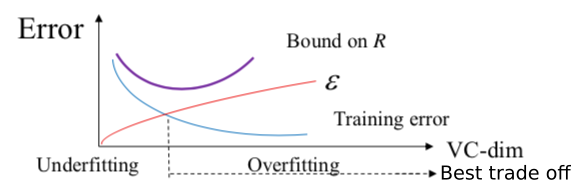
\includegraphics[scale = 0.4]{lectures/1_Introduction/intro_struct_risk.png}
\end{figure}

\begin{definition}[Model selection]
The model selection consist in choise of the model (H) with the better bound on the true risk.
\end{definition}
\begin{example}
It is possible to derive an upper bound of the ideal error which is valid with probability $(1-\delta)$, delta being arbitrarily small, of the form:
\end{example}

\begin{figure}[ht]
    \centering
    \includegraphics[scale = 0.4]{lectures/1_Introduction/intro_vc_example.png}
\end{figure}

\subsubsection{Complexity control}
SLT - Statistical Learning Theory:
\begin{itemize}
    \item It allows formal framing of the problem of generalization and overfitting, providing analytic upper-bound to the risk $R$ for the prediction over all the data, regardless to the type of learning algorithm or details of the model..
    
    \item The ML is well founded: the Learning risk can be analytically limited and only few concepts are fundamentals !
    
    \item SLT has allowed to leads to new models (e.g SVM) and other methods that directly consider the control of the complexity in the construction of the model
    
    \item bases one of the inductive principles on the control of the complexity
    
    \item explain the main difference with respect to supporting methods from CM (providing
the techniques to perform fitting), apart from modelling aspects
\end{itemize}

But there are other open questions: what (other) principles are to found the control of the complexity? How to work in practice? How to measure the complexity (or fitting flexibility)? How find the best trade-off between fitting and model complexity?

\subsection{VALIDATION}
Evaluate generalization capabilities (of your $h(x)$). \textbf{Warning}: The performance on training data provide an overoptimistic evaluation
\begin{center}
    Evaluation of performances for ML systems = Predictive accuracy
\end{center}

Validation phase has two main aims:

\begin{itemize}
    \item \textbf{Model selection}: estimating the performance (generalization error) of different learning models in order to choose the best one (to generalize).\\
    this includes search the best hyper-parameters of your model (e.g. polynomial order, ...).
    \begin{center}
        It returns a model
    \end{center}
    
    \item \textbf{Model assessment}: having chosen a final model, estimating/evaluating its prediction error/ risk (generalization error) on new test data (measure of the quality/performance of the ultimately chosen model).
    \begin{center}
        It returns an estimation
    \end{center}
\end{itemize}

\noindent\textbf{Gold rule}: Keep separation between goals and use separate data sets for this two operation.

In an ideal world, for validation we should have:

\begin{itemize}
    \item a large training set (to find the best hypothesis, see the theory)

    \item a large validation set for model selection
    
    \item a very large external unseen data test set
\end{itemize}
But with a finite and often small data set we will have just a estimation of the generalization performance. Let's see two basic techniques for validation: Simple hold-out (basic setting) and K-fold Cross Validation.

\subsubsection{Hold out cross validation}
Hold out: basic setting.\\ 
Partition data set D into training set (TR), validation or selection set (VL) and test set (TS). See figure \ref{fig:intro_cross_valid}
\begin{figure}[H]
    \centering
    \includegraphics[scale = 0.4]{lectures/1_Introduction/intro_cross_valid.png}
    \caption{Hold out cross validation}
    \label{fig:intro_cross_valid}
\end{figure}

\begin{itemize}
    \item All the three sets are disjoint sets
    \item Training is used to run the training algorithm
    \item VL can be used to select the best model (e.g hyper-parameters tuning)
    \item Test set is not to be used for tuning/selecting the best $h$: it is only for model assessment
\end{itemize}

\subsubsection{Hold out and K-fold cross validation}
\begin{figure}
    \centering
    \includegraphics[scale = 0.3]{lectures/1_Introduction/1_kfold.png}
    \caption{k-fold cross validation}
    \label{fig:1_kfold}
\end{figure}
When we have a small number of data, Hold out Cross Validation can make insufficient use of data. To solve this problem we can use another technique called: \textbf{K-fold Cross-Validation}:

\begin{itemize}
    \item Split the data set $D$ into k mutually exclusive subsets $D_1,D_2,\dots,D_k$
    \item Train the learning algorithm on $\frac{D}{D_{i}}$ and test it on $D_i$ repeat this phase k time and then we take the mean of the validation results.
    \item Can be applied for both VL or TS splitting
    \item It uses all the data for training and validation/testing
\end{itemize}

But this technique has some issues: 
\begin{itemize}
    \item How many folds? 3-fold, 5-fold , 10-fold, ...., 1-leave-out
    \item Often computationally very expensive (we have to perform training and validation phases k times)
\end{itemize}

Combinable with validation set, double-K-fold CV, ....


\subsubsection{TR/VL/TS by a schema}:
\begin{figure}[H]
    \centering
    \includegraphics[scale = 0.37]{lectures/1_Introduction/intro_cross_valid_schema.png}
    \caption{TR/VL/TS by a schema}
    \label{fig:intro_cross_valid_schema}
\end{figure}

\subsubsection{Classification Accuracy}
In the field of machine learning and specifically the problem of statistical classification, a confusion matrix, also known as an error matrix.
A confusion matrix is a table that is often used to describe the performance of a classification model (or “classifier”) on a set of test data for which the true values are known. It allows the visualization of the performance of an algorithm. See figure \ref{fig:Confusion matrix}.

\begin{figure}[H]
    \centering
    \includegraphics[scale = 0.4]{lectures/1_Introduction/intro_classification_accuracy.png}
    \caption{Confusion matrix}
    \label{fig:Confusion matrix}
\end{figure}
The number of correct and incorrect predictions are summarized with count values and broken down by each class. This is the key to the confusion matrix.
The confusion matrix shows the ways in which your classification model is confused when it makes predictions.
It gives us insight not only into the errors being made by a classifier but more importantly the types of errors that are being made.

Definition of the Terms:
\begin{itemize}
    \item Positive (P) : Observation is positive (for example: is an apple).
    \item Negative (N) : Observation is not positive (for example: is not an apple).
    \item True Positive (TP) : Observation is positive, and is predicted to be positive.
    \item False Negative (FN) : Observation is positive, but is predicted negative.
    \item True Negative (TN) : Observation is negative, and is predicted to be negative.
    \item False Positive (FP) : Observation is negative, but is predicted positive.
\end{itemize}

\noindent\textbf{Classification Rate/Accuracy} is given by the relation:
$$ \frac{TP + TN}{Total = TP + TN + FP + FN}$$ 

Two importat statistical measures are: \textit{Specificity} and \textit{Sensitivity}.

\subsubsection*{Specificity}%
Specificity (also called the true negative rate) measures the proportion of actual negatives that are correctly identified as such (e.g., the percentage of healthy people who are correctly identified as not having the condition).
$$ Specificity = \frac{TN}{FP + TN} = 1 - FPR $$
where FPR (fall-out or false positive rate) = $FP/N = FP/(FP + TN)$.

\subsubsection*{Sensitivity}
Sensitivity (also called the true positive rate, the recall, or probability of detection[1] in some fields) measures the proportion of actual positives that are correctly identified as such (e.g., the percentage of sick people who are correctly identified as having the condition).
$$ Sensitivity = \frac{TP}{TP + FN}$$

\textbf{NOTE}: for binary classif.: 50\% correctly classified = “coin” (random guess) predictor. Of course could exists trivial classifier with unbalanced data (e.g. 99\% of the data are positive).

\subsubsection*{ROC Curve}
An ROC curve (receiver operating characteristic curve) is a graph showing the performance of a classification model at all classification thresholds. This curve plots two parameters: Sensitivity (True Positive Rate (TPR)) and False Positive Rate (FPR) (1 - Specificity).

Lowering the classification threshold classifies more items as positive, thus increasing both False Positives and True Positives. See figure \ref{fig:intro_roc_curve_1}.

\begin{figure}[ht]
  \centering
  \subfloat[AUC (Area under the ROC Curve)]{\includegraphics[width=0.5\textwidth]{lectures/1_Introduction/intro_roc_curve_2.png}\label{fig:intro_roc_curve_1}}
  \hfill
  \subfloat[AUC]{\includegraphics[width=0.5\textwidth]{lectures/1_Introduction/intro_roc_curve.png}\label{fig:intro_roc_curve_2}}
  \caption{ROC curve}
\end{figure}
\textbf{AUC} stands for "Area under the ROC Curve." and measures the entire two-dimensional area underneath the entire ROC curve (think integral calculus) from (0,0) to (1,1). See figure \ref{fig:intro_roc_curve_2}.

AUC provides an aggregate measure of performance across all possible classification thresholds. One way of interpreting AUC is as the probability that the model ranks a random positive example more highly than a random negative example.

The diagonal corresponds to the worst classifier (random guessing). Better curves have higher AUC (Area Under the Curve). In $1.0$ we have the perfect classification.

\subsection{The Design Cycle}
\noindent\textbf{Data collection:} adequately large and representative set of examples for training and test the system

\noindent\textbf{Data representation:} Often the most critical phase for an overall success.
\begin{itemize}
    \item domain dependent, exploit prior knowledge of the application expert
    \item Feature selection
    \item Outliers detection
    \item Other preprocessing: variable scaling, missing data,..
\end{itemize}

\noindent\textbf{Model choice:}
\begin{itemize}
    \item Statement of the problem.
    \item Hypothesis formulation: You must know the limits of applicability of your model.
    \item Complexity control.
\end{itemize}
\noindent\textbf{Building of the model (core of ML):} through the learning algorithm using the training data.

\noindent\textbf{Evaluation:} performance = predictive accuracy.

\begin{figure}[ht]
    \centering
    \includegraphics[scale = 0.3]{lectures/1_Introduction/intro_design_cycle.png}
    \caption{Design cycle}
    \label{fig:intro_design_cycle}
\end{figure}

\subsection{Misinterpretations}
For every statistical models (including Data Mining (DM) applications).

\noindent Causality is (often) assumed and a set of data representative of the phenomena is needed.
\begin{itemize}
    \item Not for unrelated variables and for random phenomena (lotteries)
    \item Uninformative input variables $\rightarrow$ poor modeling $\rightarrow$ Poor learning results
\end{itemize}

\noindent Causality cannot be inferred from data analysis alone:
\begin{itemize}
    \item People in Florida are older(on av.) than in other US states.
    \item Florida climate causes people to live longer ?
\end{itemize}

\noindent May be there is a statistical dependencies for reasons outside the data.

\noindent More specifically for ML:
\begin{itemize}
    \item Powerful models (even for “garbage” data) $\rightarrow$ higher risk !
    \item Not-well validated results: the predicted outcome and the interpretation can be misleading.
\end{itemize}

\end{document}
    
